\section{Basic Semiconductor Device Structures}
\subsection{pn Junction --- pn Diode}
\begin{itemize}
        \item Carriers recombine and a \textbf{space charge region} (SCR) with an elec. field $\vec{E}$ arises
  \item At thermal equilibrium:
        \begin{align*}
          &\vec{j}_{n, \mathrm{drift}} = \vec{j}_{n, \mathrm{diff}}\\
          &\vec{j}_{n}(\vec{r}) = en\mu_{n}\vec{E} + \mu_{n}kT\,\nabla n = 0\\
          &\vec{j}_{p}(\vec{r}) = en\mu_{p}\vec{E} - \mu_{p}kT\,\nabla p = 0
        \end{align*}
\end{itemize}

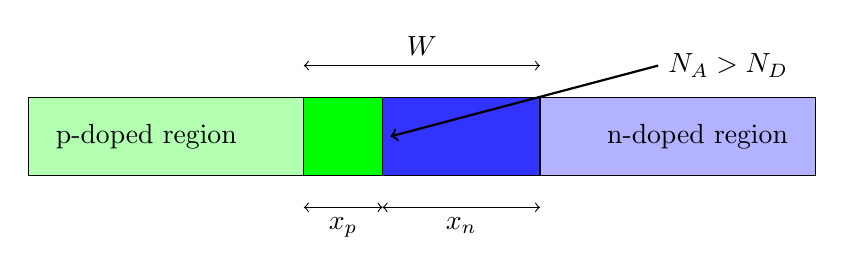
\begin{tikzpicture}
  \pgfmathsetmacro{\pnJunction}{4.5};
  \pgfmathsetmacro{\scrLeft}{3.5};
  \pgfmathsetmacro{\scrRight}{6.5};
  %% Semiconductor blocks
  \filldraw[draw=black!, fill=green!30] (0,0) rectangle (\pnJunction,1);
  \filldraw[draw=black!, fill=blue!30] (\pnJunction,0) rectangle (10,1);
  \draw (1.5,.5) node[]{p-doped region};
  \draw (8.5,.5) node[]{n-doped region};
  %% Space Charge Region (SCR)
  \filldraw[draw=black!, fill=green!] (\scrLeft,0) rectangle (\pnJunction,1);
  \filldraw[draw=black!, fill=blue!80] (\pnJunction,0) rectangle (\scrRight,1);
  %% Measurements
  \draw[<->] (\scrLeft, 1.4) -- node[above]{$W$} (\scrRight, 1.4);
  \draw[<->] (\scrLeft, -.4) -- node[below]{$x_{p}$} (\pnJunction, -.4);
  \draw[<->] (\pnJunction, -.4) -- node[below]{$x_{n}$} (\scrRight, -.4);
  %% Label
  \draw[->, thick] (8, 1.4) node[right]{$N_{A} > N_{D}$} -- (\pnJunction + .1, .5);
\end{tikzpicture}

\begin{align*}
  &x_{p} \cdot N_{A} = x_{n} \cdot N_{D} & \text{: charge neutrality}\\
  &W = x_{p} + x_{n} & \text{: width of depletion region}
\end{align*}

\begin{itemize}
        \item Abrupt pn junctions block more voltage
\end{itemize}

\subsection{Metal-Semiconductor Junctions}
\begin{itemize}
  \item Application as diodes with low threshold voltage and ohmic contacts
  \item Properties of Schottky diodes:
        \begin{itemize}
          \item current carried by majority carriers
          \item $V_{th}$ lower than in pn diodes
          \item fast switching time (application in fast logic and HF circuits)
          \item \textcolor{red}{But:} higher reverse current and lower blocking capability
        \end{itemize}
  \item Schottky diodes as freewheeling diodes (low junction voltage)
  \item Schottky diodes with wide-bandgap materials for better blocking
        \begin{equation*}
          j = j_{s} \cdot \left(\exp\left[\dfrac{qV_{f}}{kT}\right] - 1\right), \quad j_{s} = \underbrace{A^{*}}_{\text{Richardson const.}}\, T^{2} \exp\left(\dfrac{-q V_{B}}{kT}\right)
        \end{equation*}
    \item For ohmic contacts: highly doped semiconductors are used, creating a thinner barrier $\implies$ tunneling of electron possible
\end{itemize}

\section{Bipolar Transistor}
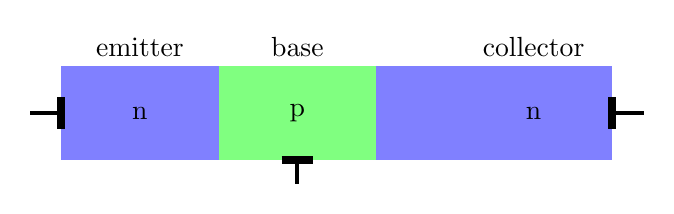
\begin{tikzpicture}
  %% Conveniant macros for adjusting size later
  \pgfmathsetmacro{\blockHeight}{1.2}
  \pgfmathsetmacro{\blockLength}{7}
  \pgfmathsetmacro{\emitterBaseJunction}{2}
  \pgfmathsetmacro{\baseCollectorJunction}{4}
  \pgfmathsetmacro{\baseMiddle}{(\emitterBaseJunction + \baseCollectorJunction) / 2}
  %% npn-blocks
  \fill[fill=blue!50] (0,0) rectangle (\emitterBaseJunction, \blockHeight);
  \fill[fill=green!50] (\emitterBaseJunction,0) rectangle (\baseCollectorJunction, \blockHeight);
  \fill[fill=blue!50] (\baseCollectorJunction, 0) rectangle (\blockLength, \blockHeight);
  %% Contacts
  \draw[line width=1mm] (0,\blockHeight / 2 + .2) -- (0,\blockHeight / 2 - .2);
  \draw[line width=.5mm] (0,\blockHeight / 2) -- (-.4,\blockHeight / 2);
  \draw[line width=1mm] (\blockLength,\blockHeight / 2 + .2) -- (\blockLength,\blockHeight / 2 - .2);
  \draw[line width=.5mm] (\blockLength,\blockHeight / 2) -- (\blockLength + .4,\blockHeight / 2);
  \draw[line width=1mm] (\baseMiddle - .2,0) -- (\baseMiddle + .2,0);
  \draw[line width=.5mm] (\baseMiddle,0) -- (\baseMiddle,-.3);
  %% Labels
  \draw (1,\blockHeight) node[above]{emitter};
  \draw (1,\blockHeight / 2) node[]{n};
  \draw (3,\blockHeight) node[above]{base};
  \draw (3,\blockHeight / 2) node[]{p};
  \draw (6,\blockHeight) node[above]{collector};
  \draw (6,\blockHeight / 2) node[]{n};
\end{tikzpicture}
\begin{itemize}
  \item Electrons injected by emitter into base
        \begin{itemize}
                \item partially recombine with holes $\implies$ holes are replaced via base current
                \item $l_{\mathrm{diff}} > w_{b}$: diffusion of electrons into collector region $\implies I_{c}$
        \end{itemize}
        \item Small changes in base current $\implies$ large impact on collector current
\end{itemize}

\section{MOS Structure --- MOS Field Effect Transistor}
